\chapter{Results}
\label{chap:results}

\section{Phase and milestone summary}
\label{sec:phase_and_milestone_summary}

\begin{longtable}{@{}p{0.313\textwidth} p{0.313\textwidth} p{0.313\textwidth}@{}}
\caption{Phase and milestone summary: structured summary}\\
\toprule
\textbf{Phase} & \textbf{Principal output} & \textbf{Status} \\
\midrule
\endfirsthead
\toprule
\textbf{Phase} & \textbf{Principal output} & \textbf{Status} \\
\midrule
\endhead
0 & Immutable paired data model and scientific contract & M0 passed \\
1 & QC, missingness atlas and frozen 42/35-pair cohorts & M1 passed \\
2 & Missingness/imputation/PCA benchmark & \textbf{Not implemented} \\
3 & Paired abundance and detection inference & Computational branch passed; M3 conditional on Phase 2 \\
4 & Reactome interpretation and heterogeneity & Computational checks passed; M4 conditional \\
5 & Leakage-safe AI and stability catalogue & Computational checks passed; no compact panel; M5 conditional \\
6 & Multiverse, patient influence and integrated evidence & Implemented; M6 open pending Phase 2 and independent clean rebuild \\
7 & Validation-readiness and locked hand-off & Readiness passed; validation not executed \\
\bottomrule
\end{longtable}

\section{Data audit}
\label{sec:data_audit}

The source contains 8,071 feature rows and 84 unique specimens forming exactly 42 patient pairs. All 437,584 observed values are finite and positive; no pseudocount was required. There are 240,380 blanks, giving 35.456\% missingness. Observed values range from 0.002342 to approximately 7.311 billion, supporting interpretation as positive linear-scale quantities rather than conventional log2 values.

There are 114 entirely unobserved rows, eight rows belonging to four duplicated labels (\texttt{\detokenize{CDKN2A}}, \texttt{\detokenize{CUX1}}, \texttt{\detokenize{MOCS2}}, \texttt{\detokenize{TMPO}}) and 48 semicolon-delimited compound labels. Of 8,071 rows, 7,239 have at least one complete quantitative pair, 832 have none and 1,350 are complete across all 42 pairs. Across 338,982 patient-feature states, 176,223 are detected in both tissues, 18,605 only in matched non-tumour, 66,533 only in tumour and 77,621 in neither.

\section{Quality control and missingness}
\label{sec:quality_control_and_missingness}

Matched non-tumour specimens contain a median 4,759 detected features (range 2,460–6,549); tumour specimens contain a median 5,919.5 (range 4,463–6,370). Tumour coverage exceeds matched non-tumour coverage in 37/42 pairs. The median paired coverage difference is 1,023 features.

Observed log2 abundance medians move oppositely: 13.084 in matched non-tumour and 12.552 in tumour. Coverage and observed median abundance have pooled Spearman rho −0.914, indicating that missingness and observed abundance structure are strongly related without proving a specific mechanism.

\begin{figure}[p]
\centering
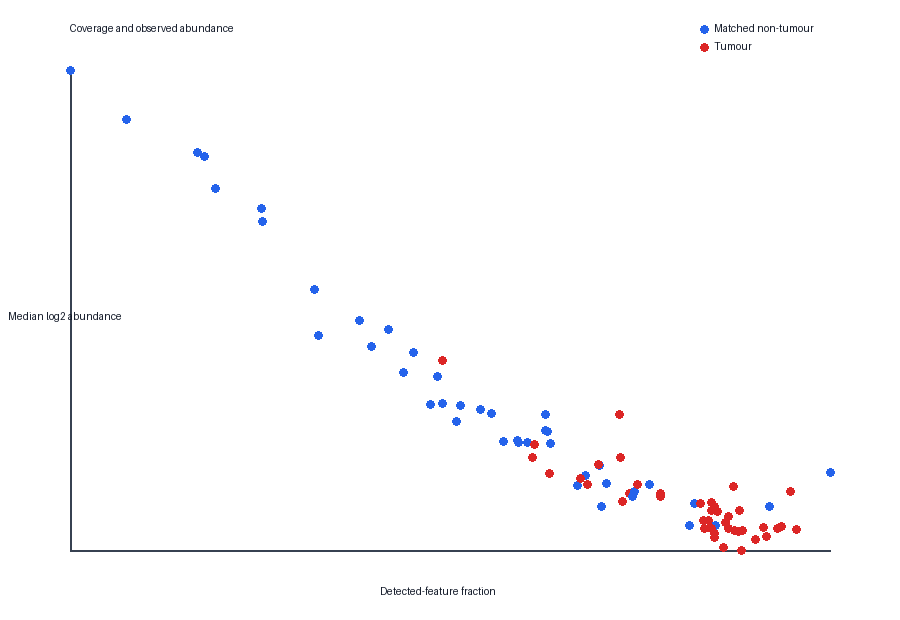
\includegraphics[width=0.96\textwidth,height=0.78\textheight,keepaspectratio]{figures/coverage_vs_median.png}
\caption{Specimen detection coverage versus median observed log2 abundance. The strong inverse association motivates separate abundance and detection analyses.}
\label{fig:coverage_vs_median}
\end{figure}

Missingness decreases from 78.64\% in the lowest observed-abundance decile to 4.45\% in the highest. Tumour detection fractions exceed matched non-tumour fractions for 5,413 rows; the reverse occurs for 986 rows and equality for 1,672.

\begin{figure}[p]
\centering
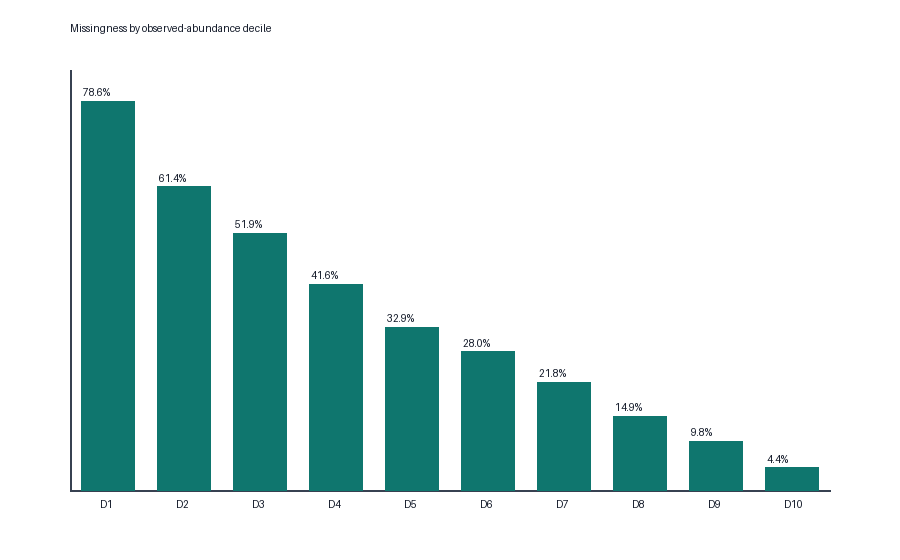
\includegraphics[width=0.96\textwidth,height=0.78\textheight,keepaspectratio]{figures/missingness_by_abundance_decile.png}
\caption{Mean missingness across observed-abundance deciles, showing strong abundance dependence.}
\label{fig:missingness_by_abundance_decile}
\end{figure}

The median within-pair detection Jaccard similarity is 0.708 (range 0.371–0.880), the median pairwise Spearman correlation is 0.745 (range 0.367–0.940), and the median absolute paired log2 difference is 0.734 (range 0.301–1.521).

\begin{figure}[p]
\centering
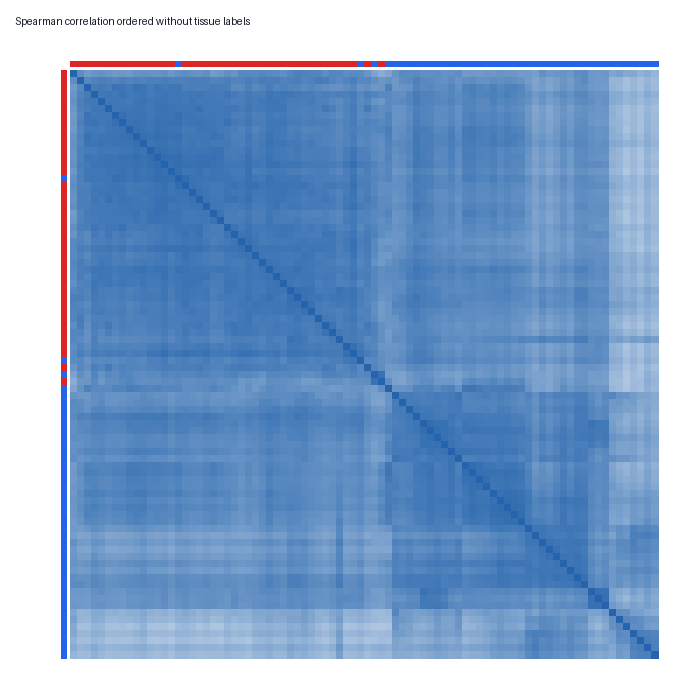
\includegraphics[width=0.96\textwidth,height=0.78\textheight,keepaspectratio]{figures/sample_correlation_heatmap.png}
\caption{Pairwise-complete sample Spearman correlation heatmap with label-blind clustering order.}
\label{fig:sample_correlation_heatmap}
\end{figure}

Diagnostic PCA explains 20.07\% on PC1 and 9.89\% on PC2; the first five components explain 46.75\%. Tissue centroids differ strongly, but batch, purity, inflammation and sampling metadata are unavailable.

\begin{figure}[p]
\centering
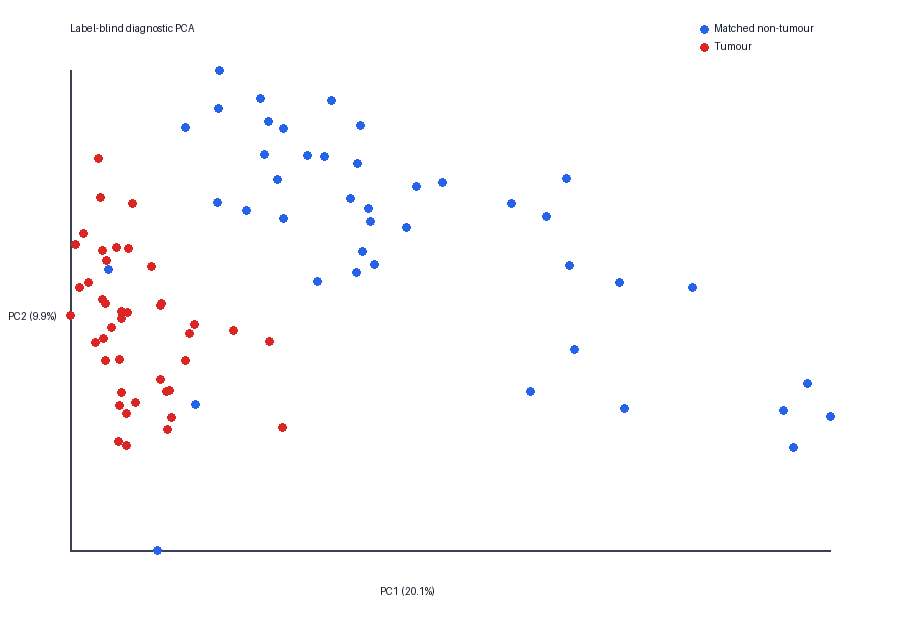
\includegraphics[width=0.96\textwidth,height=0.78\textheight,keepaspectratio]{figures/pca_qc.png}
\caption{Label-blind QC PCA of high-coverage features. Tissue annotations were attached after calculation.}
\label{fig:pca_qc}
\end{figure}

Twelve specimens from seven patients (\texttt{\detokenize{P1}}, \texttt{\detokenize{P2}}, \texttt{\detokenize{P19}}, \texttt{\detokenize{P21}}, \texttt{\detokenize{P25}}, \texttt{\detokenize{P31}}, \texttt{\detokenize{P42}}) meet the two-family sensitivity flag rule. All 42 pairs remain primary; the frozen sensitivity cohort contains 35 pairs.

\section{Paired feature inference}
\label{sec:paired_feature_inference}

The primary abundance rule admits 3,430 features. The empirical-Bayes variance prior has 3.776 prior degrees of freedom and scale 0.718. At BH q≤0.05, 2,194 features have quantitative evidence: 986 positive and 1,208 negative. Adding the effect, direction and support thresholds yields 669 primary core features. Cross-scenario stability and identifier requirements leave 614 \texttt{\detokenize{B_abundance}} candidates: 128 positive and 486 negative.

Examples include PRELP (mean log2 difference −5.346; moderated 95\% interval −6.052 to −4.640) and SERPINH1 (2.425; interval 2.091–2.760). Other precise candidates include OGN, SLC3A2, HSPH1, ALDH9A1, EPHX1, PEBP1, SOD3 and DDAH2.

\begin{figure}[p]
\centering
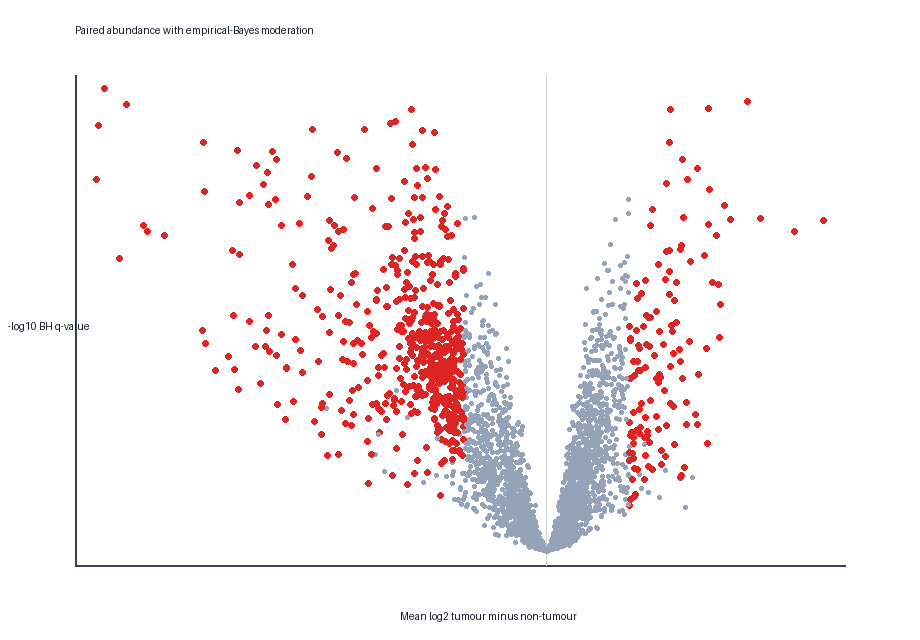
\includegraphics[width=0.96\textwidth,height=0.78\textheight,keepaspectratio]{figures/abundance_volcano.png}
\caption{Paired abundance effects and BH-adjusted evidence. Highlighting follows the frozen abundance-core rule.}
\label{fig:abundance_volcano}
\end{figure}

For detection, 2,887 rows have BH q≤0.05; 2,549 meet the primary effect and discordance rule; and 1,831 remain stable in the unflagged cohort. Among these stable patterns, 1,695 favour tumour detection and 136 favour matched non-tumour detection. After excluding ambiguous identifiers, 1,827 rows receive \texttt{\detokenize{C_detection_pattern}}. Leading tumour-detection labels include SLC38A2, NEDD1, KPNA7, NCAPG, NOMO1, HMGA2, WDR75, SLC38A5, POP4 and SLC39A14.

\begin{figure}[p]
\centering
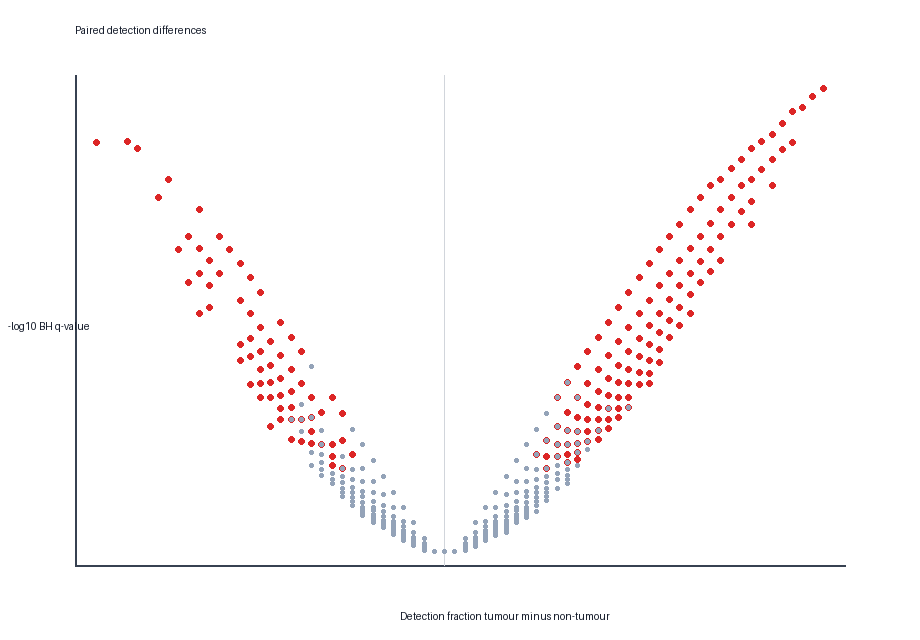
\includegraphics[width=0.96\textwidth,height=0.78\textheight,keepaspectratio]{figures/detection_volcano.png}
\caption{Paired detection-fraction differences and BH-adjusted exact-test evidence.}
\label{fig:detection_volcano}
\end{figure}

No feature meets the strict \texttt{\detokenize{A_concordant}} rule. This is structurally plausible because quantitative eligibility requires many both-observed pairs, whereas strong detection evidence requires many discordant pairs. The branches are complementary rather than failed replicas of one another.

\section{Pathway organisation}
\label{sec:pathway_organisation}

The ranked view tests 783 pathways, with 328 passing BH q≤0.05. The patient-score view tests 749 pathways, with 566 passing. There are 271 pathways supported by both views with consistent direction.

Positive organisation includes capped-intron pre-mRNA processing (NES 3.297; ranked q=0.00559; paired mean score 0.831; score q=0.000161), mRNA splicing (NES 3.261; mean score 0.865), translation (NES 2.253; mean score 0.438), antigen processing–cross presentation (NES 2.151; mean score 0.352) and cytokine signalling (NES 2.236; mean score 0.257).

Negative organisation includes citric-acid-cycle/respiratory-electron transport (NES −2.835; mean score −1.165), respiratory electron transport (NES −2.869; mean score −1.242), collagen degradation (NES −2.082; mean score −0.723), extracellular-matrix degradation (NES −1.974; mean score −0.629), complement cascade (NES −2.129; mean score −0.550) and haemostasis (NES −1.440; mean score −0.323).

\begin{figure}[p]
\centering
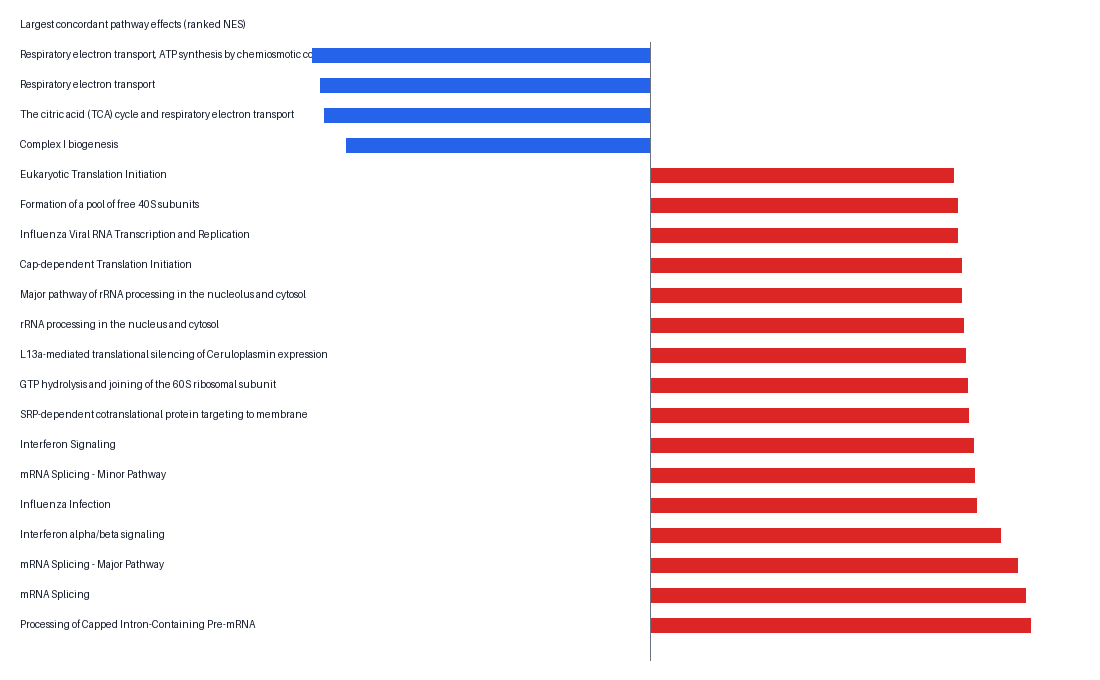
\includegraphics[width=0.96\textwidth,height=0.78\textheight,keepaspectratio]{figures/pathway_evidence.png}
\caption{Largest concordant ranked pathway effects. Pathway names organise measured proteins and do not prove pathway activation or causality.}
\label{fig:pathway_evidence}
\end{figure}

\section{Patient heterogeneity}
\label{sec:patient_heterogeneity}

Among 1,350 complete paired-difference features, 500 variable rows entered robust PCA. PC1 explains 41.41\% (bootstrap median 42.20\%, interval 29.83–52.42\%) and PC2 16.13\% (median 17.42\%, interval 11.72–24.25\%). Four components explain 70.72\%. Large PC1 loadings include mitochondrial and metabolic proteins such as CYC1, UQCRB, NDUFV1, NDUFS3, SDHB, OGDH and DLD.

\begin{figure}[p]
\centering
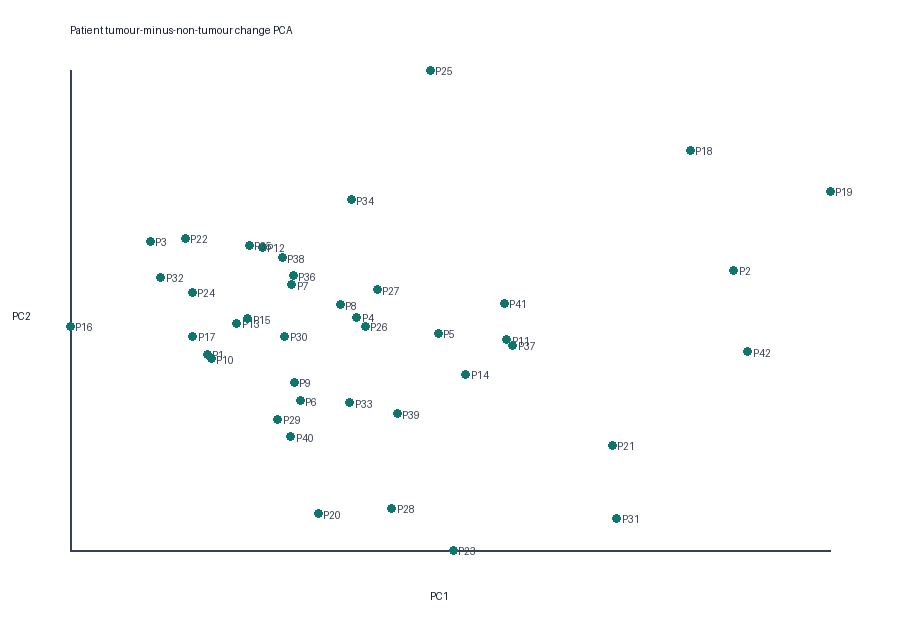
\includegraphics[width=0.96\textwidth,height=0.78\textheight,keepaspectratio]{figures/patient_change_pca.png}
\caption{PCA of patient-level tumour-minus-non-tumour change profiles.}
\label{fig:patient_change_pca}
\end{figure}

No consensus-clustering solution passes all frozen criteria. The least ambiguous exploratory \texttt{\detokenize{k=2}} solution contains 12 and 30 patients, with PAC 0.261, mean within-cluster consensus 0.934 and silhouette 0.372. Because PAC exceeds 0.10, no clinical or molecular subtype is accepted.

\begin{figure}[p]
\centering
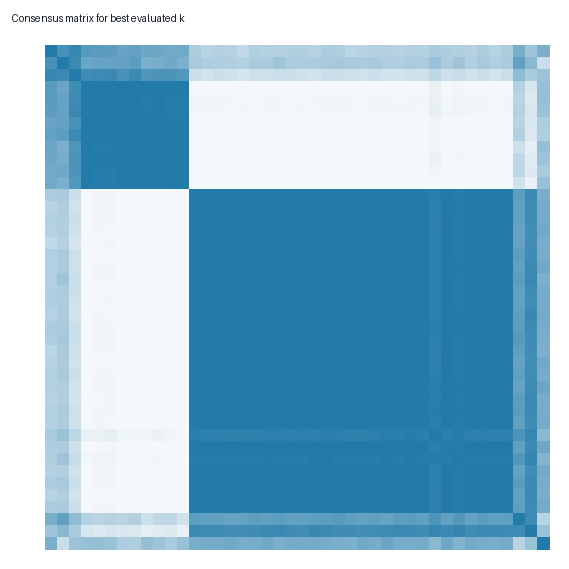
\includegraphics[width=0.96\textwidth,height=0.78\textheight,keepaspectratio]{figures/consensus_clustering.png}
\caption{Consensus matrix for the best exploratory \texttt{\detokenize{k}}; it remains unstable under the prespecified PAC criterion.}
\label{fig:consensus_clustering}
\end{figure}

\section{Machine-learning performance}
\label{sec:machine_learning_performance}

Across 25 repeated nested partitions, the main results are:

\begin{longtable}{@{}p{0.235\textwidth} p{0.235\textwidth} p{0.235\textwidth} p{0.235\textwidth}@{}}
\caption{Machine-learning performance: structured summary}\\
\toprule
\textbf{Pipeline} & \textbf{Median ROC AUC} & \textbf{Median balanced accuracy} & \textbf{Interpretation} \\
\midrule
\endfirsthead
\toprule
\textbf{Pipeline} & \textbf{Median ROC AUC} & \textbf{Median balanced accuracy} & \textbf{Interpretation} \\
\midrule
\endhead
Abundance elastic net & 0.982 & 0.964 & Highest median AUC; dense model \\
Abundance linear SVM & 0.980 & 0.964 & Similar performance \\
Combined elastic net & 0.974 & 0.952 & No improvement over abundance \\
Combined linear SVM & 0.974 & 0.952 & No improvement over abundance \\
Detection elastic net & 0.954 & 0.940 & Strong but lower discrimination \\
Detection linear SVM & 0.960 & 0.940 & Strong detection view \\
Fold-local PCA logistic & 0.969 & 0.940 & Close low-dimensional baseline \\
Coverage logistic & 0.868 & 0.786 & Coverage contains substantial signal \\
Intercept null & 0.500 & 0.500 & Chance baseline \\
\bottomrule
\end{longtable}

\begin{figure}[p]
\centering
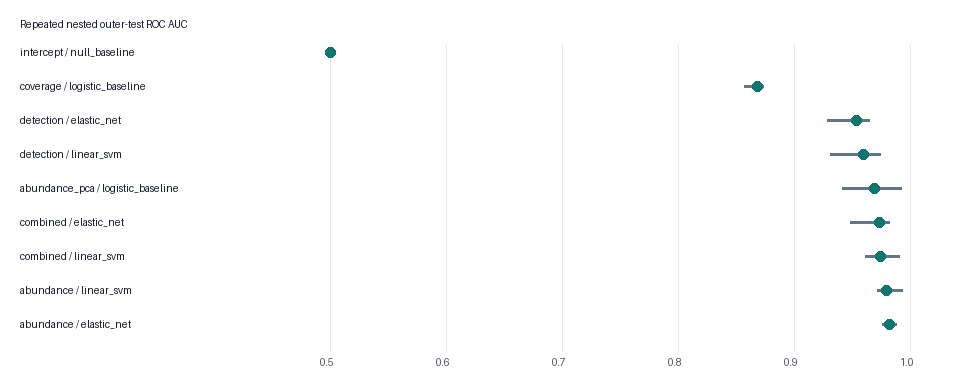
\includegraphics[width=0.96\textwidth,height=0.78\textheight,keepaspectratio]{figures/nested_auc_summary.png}
\caption{Outer-test ROC AUC distributions from repeated patient-grouped nested validation.}
\label{fig:nested_auc_summary}
\end{figure}

The abundance elastic-net median sensitivity is 0.976 and specificity 0.952. However, median calibration intercept is −0.406 and slope 3.53, showing that probability calibration is not transportable. The fold-local PCA baseline has better Brier behaviour and only modestly lower discrimination, so the high-dimensional model does not represent a wholly distinct predictive capability.

The observed paired-label permutation AUC is 0.9768. Across 200 complete nested null reruns, the median is approximately 0.4786 and maximum 0.7319, producing empirical p=(1+0)/(200+1)=0.004975.

\begin{figure}[p]
\centering
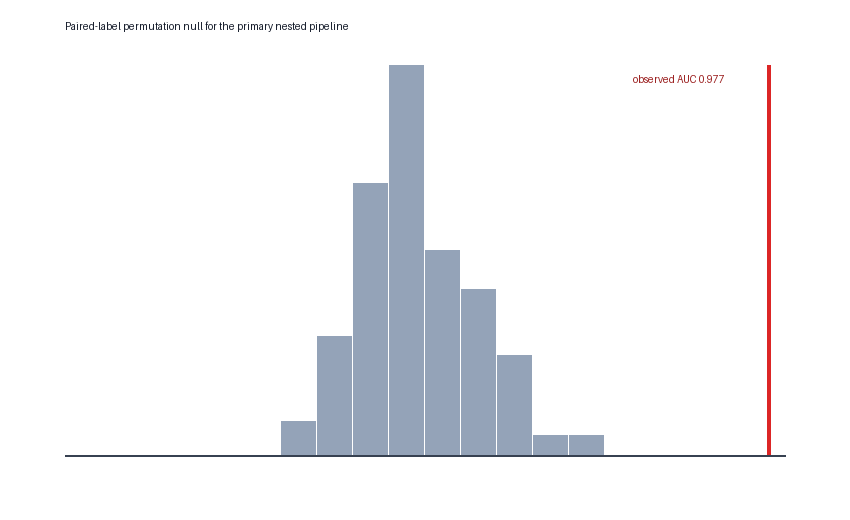
\includegraphics[width=0.96\textwidth,height=0.78\textheight,keepaspectratio]{figures/paired_permutation_null.png}
\caption{Full nested paired-label permutation null for the frozen combined elastic-net pipeline.}
\label{fig:paired_permutation_null}
\end{figure}

The tuned elastic nets have median selected size 97 and favour L1 ratio 0.1, behaving largely as grouped/ridge-like models. Phase 5 therefore does not declare a compact panel. There are 222 stable elastic-net view-feature rows, representing 148 unique modality-qualified features; only 70 have positive mean held-out permutation importance. Frequently recurrent rows include SERPINH1, PRELP, HSPH1, NEDD1, GNA11, MAOB, COLGALT1, OGN, SPTAN1, SLC3A2, NOMO1 and SLC38A2.

\section{Phase 6 robustness}
\label{sec:phase_6_robustness}

Across 8,071 source rows, 3,077 have complete effect-sign agreement wherever eligible, 1,757 receive FDR support in at least 80\% of eligible scenarios, and 368 meet the full core rule in at least 80\%. Core counts vary from approximately 319 under the strict uncentred/unflagged/35-pair scenario to approximately 1,050 under median-centred/all-pair/20-pair scenarios. This demonstrates real sensitivity to analysis choice.

\begin{figure}[p]
\centering
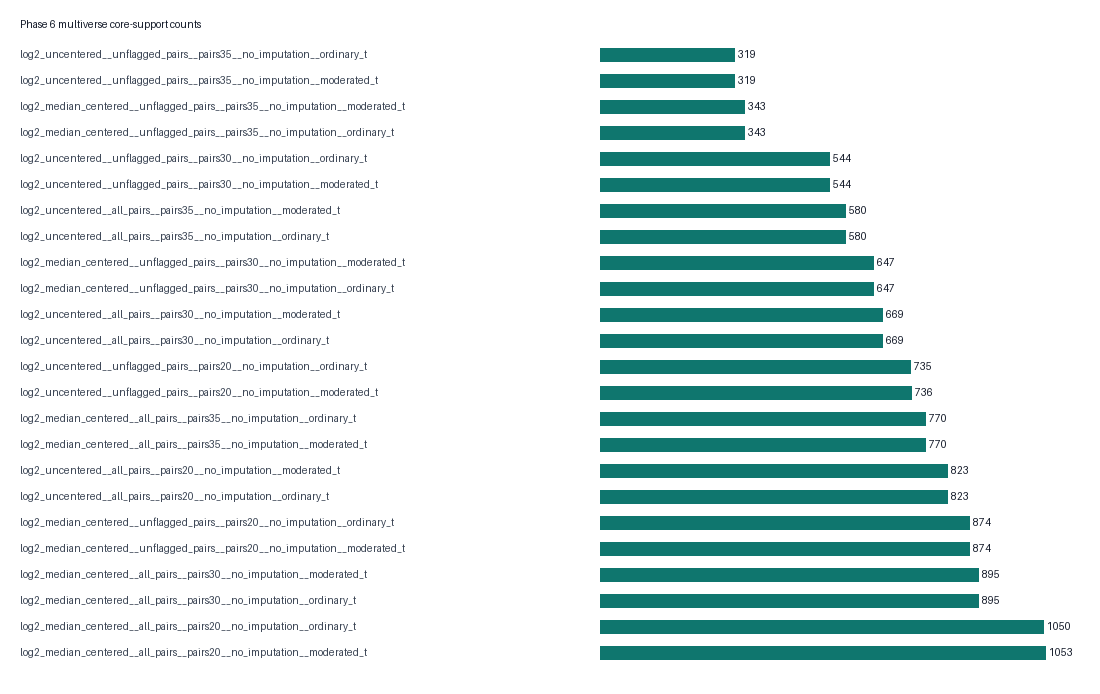
\includegraphics[width=0.96\textwidth,height=0.78\textheight,keepaspectratio]{figures/multiverse_core_support.png}
\caption{Core feature counts across the 24 prespecified multiverse scenarios.}
\label{fig:multiverse_core_support}
\end{figure}

Exact leave-one-patient-out inference shows that 583/614 abundance candidates and 1,804/1,827 detection candidates retain core support in at least 80\% of omissions. None of the 614 abundance candidates reverses effect direction. Exact grouped leave-one-patient-out abundance elastic net yields AUC 0.9847, balanced accuracy 0.9643 and correct orientation for 41/42 pairs.

Of 783 pathways, 596 meet direction agreement ≥80\% and median leading-edge Jaccard ≥0.30; 563 preserve identical direction across every scenario. The observed overlap between Phase 3 tiered candidates and stable Phase 5 ML features is 140. In 1,000 random feature-key permutations, the median is 45 and maximum 64, giving empirical p=0.000999. This indicates non-random convergence within the dataset, not independent replication.

Frozen integration classifies 165 rows as \texttt{\detokenize{high_priority_internal}}, 1,909 as \texttt{\detokenize{robust_single_domain}}, 28 as \texttt{\detokenize{predictive_stability_only}} and 5,969 as \texttt{\detokenize{not_prioritized}}. The high-priority group contains 107 abundance and 58 detection candidates.

\begin{figure}[p]
\centering
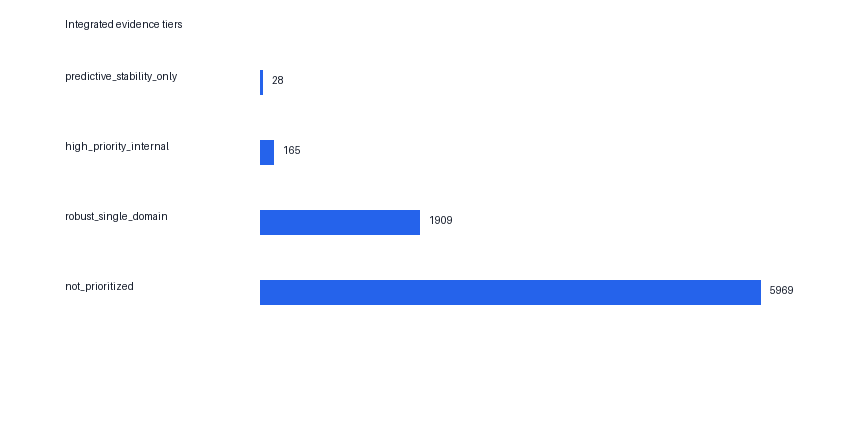
\includegraphics[width=0.96\textwidth,height=0.78\textheight,keepaspectratio]{figures/integrated_evidence_tiers.png}
\caption{Counts under the frozen integrated evidence rules.}
\label{fig:integrated_evidence_tiers}
\end{figure}

\section{Phase 7 validation-readiness package}
\label{sec:phase_7_validation_readiness_package}

The 107 abundance candidates form 66 correlation components at absolute Spearman rho ≥0.80 with at least 25 complete pairs. There are 58 singleton components, four size-two components, two size-three components, one size-four component and one size-31 component. This large component illustrates extensive predictor redundancy.

\begin{figure}[p]
\centering
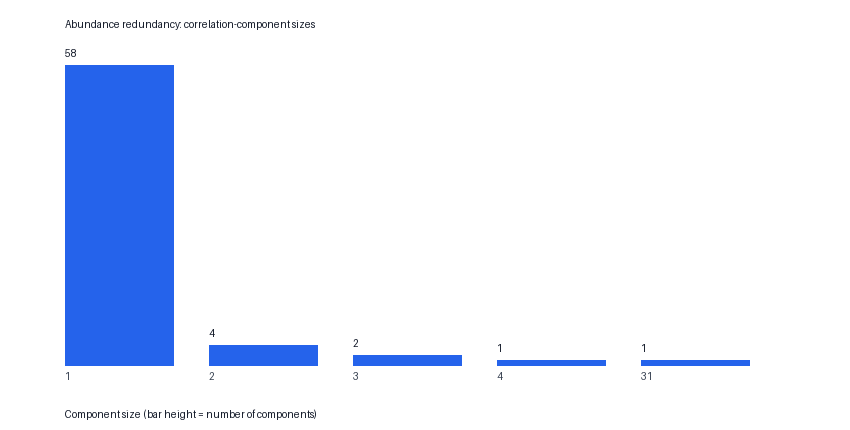
\includegraphics[width=0.96\textwidth,height=0.78\textheight,keepaspectratio]{figures/abundance_redundancy_components.png}
\caption{Distribution of abundance correlation-component sizes.}
\label{fig:abundance_redundancy_components}
\end{figure}

The abundance branch contains 14 Pareto fronts, with ten candidates on front 1. The detection branch contains ten fronts, with two candidates on front 1.

\begin{figure}[p]
\centering
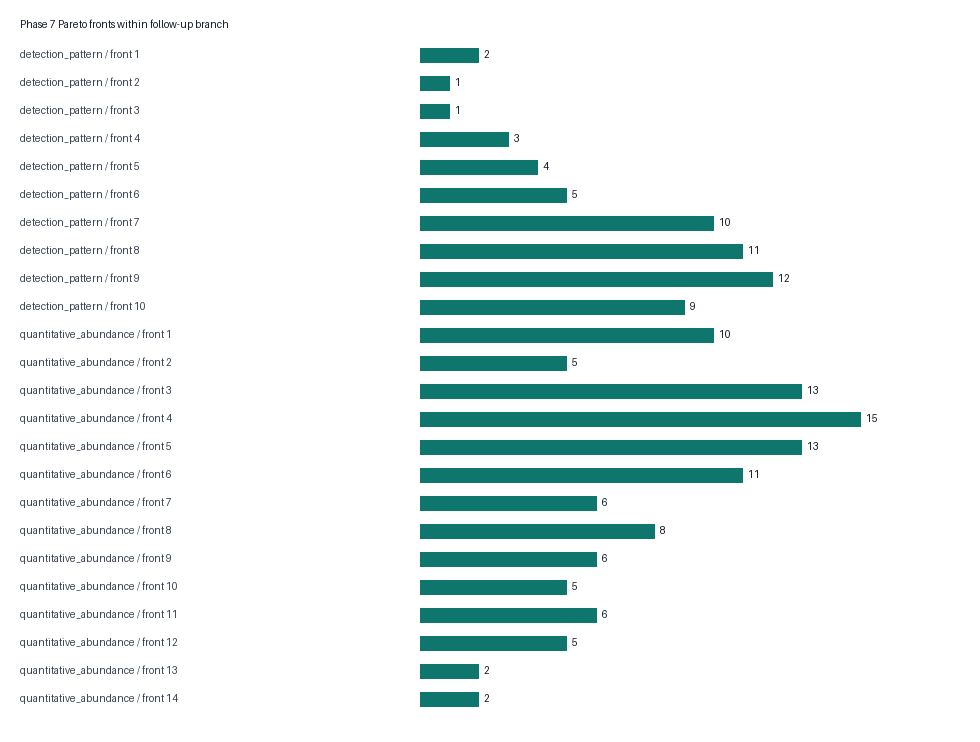
\includegraphics[width=0.96\textwidth,height=0.78\textheight,keepaspectratio]{figures/pareto_fronts.png}
\caption{Candidate counts by branch-specific nondominated Pareto front.}
\label{fig:pareto_fronts}
\end{figure}

The locked hand-off contains:

\begin{longtable}{@{}p{0.470\textwidth} p{0.470\textwidth}@{}}
\caption{Phase 7 validation-readiness package: structured summary}\\
\toprule
\textbf{Role} & \textbf{Source labels} \\
\midrule
\endfirsthead
\toprule
\textbf{Role} & \textbf{Source labels} \\
\midrule
\endhead
Quantitative-abundance replication anchors & PRELP, CMA1, MGLL, SERPINH1, SOD3, TNXB, KRT4, NDRG2, TNC, OGN, PEBP1, MAOB \\
Detection-mechanism sentinels & NEDD1, SLC38A2, KPNA7, NCAPG, HMGA2, NOMO1, WDR75, POP4 \\
\bottomrule
\end{longtable}

For the 12 abundance targets and Bonferroni planning alpha 0.004167, an assumed standardised paired effect of 0.50 requires 60 complete pairs at 80\% power or 73 at 90\%; an effect of 0.30 requires 157 or 196 pairs. These values demonstrate how strongly planning depends on the assumed replication effect. Detection planning varies additionally with total discordance; for an absolute difference of 0.20 at 80\% power, approximate requirements range from 61 pairs at discordance 0.20 to 189 at discordance 0.60.
